%%%%%%%%%%%%%%%%%%%%%%%%%%%%%%%%%%%%%%%%%%%%%%%%
%% Intro to LaTeX and Template for Homework Assignments
%% Quantitative Methods in Political Science
%% University of Mannheim
%% Fall 2018
%%%%%%%%%%%%%%%%%%%%%%%%%%%%%%%%%%%%%%%%%%%%%%%%

% created by Marcel Neunhoeffer & Sebastian Sternberg


% Every .tex file usually consists of four parts.
% 1. Document Class
% 2. Packages
% 3. Header
% 4. Your Document
 
\documentclass[a4paper,12pt]{article} % This defines the style of your paper

%%%%%%%%%%%%%%%%%%%%%%%%%%%%%%%%%%%%%%%%%%%%%%%%
% 2. Packages
%%%%%%%%%%%%%%%%%%%%%%%%%%%%%%%%%%%%%%%%%%%%%%%%

% Packages are libraries of commands that LaTeX can call when compiling the document.
% If the packages we call are not installed yet, TeXworks will ask you to install the necessary packages while compiling.
\usepackage[top = 2.5cm, bottom = 2.5cm, left = 2.5cm, right = 2.5cm]{geometry} %margins
\usepackage[T1]{fontenc}
\usepackage[utf8]{inputenc}
\usepackage{hyperref}
\usepackage{tikz} %for the flow chart
\usetikzlibrary{shapes,arrows}
\usepackage{amsmath} %math package
\usepackage{amsmath, nccmath} %multiple fractions
\usepackage{pgfplots} %plots
\usepackage{pgfplotstable} %to plot from imported text files
\pgfplotsset{compat = newest}
\usepackage{subcaption} %figures with multiple captions
\usepackage{multirow} % Multirow is for tables with multiple rows within one cell.
\usepackage{booktabs} % For even nicer tables.
\usepackage{graphicx} %to include some plots (.pdf files) we need a package for that.
\usepackage[justification=centering]{caption} %Centering captions under the figures
\usepackage{setspace}
\setlength{\parindent}{0in} %The following command sets the indent to 0.
\usepackage{float} % Package to place figures where you want them.
\usepackage{fancyhdr} % to create nice headers.
\usepackage[numbered, framed]{mcode} %Package for Matlab code listings:
\lstset{stepnumber  = 5, % Line numbers go in steps of 4
	breaklines  = true,
	breakautoindent=true, 
	breakindent=10pt,
	breakatwhitespace   = false,
	prebreak= \space,
	postbreak   = \space}

\newcommand{\tagg}[1]{%
	\tikz[baseline]\node[anchor=base,
	draw=gray!30,
	rounded corners,
	inner xsep=1ex,
	inner ysep =0.75ex,
	text height=1.5ex,
	text depth=.25ex]{#1};
  }


%%%%%%%%%%%%%%%%%%%%%%%%%%%%%%%%%%%%%%%%%%%%%%%%
% 3. Header (and Footer)
%%%%%%%%%%%%%%%%%%%%%%%%%%%%%%%%%%%%%%%%%%%%%%%%
\pagestyle{fancy} % % To make our document nice we want a header and number the pages in the footer. With this command we can customize the header style.
\fancyhf{} % This makes sure we do not have other information in our header or footer.
\lhead{\footnotesize Crop Wars}% \lhead puts text in the top left corner. \footnotesize sets our font to a smaller size. \rhead works just like \lhead (you can also use \chead)
\rhead{\footnotesize Golling, Mourouga, Moser, Schmidt, Author 5} %<---- Fill in your lastnames.
\cfoot{\footnotesize \thepage} % We want to put our page number in the center.

%%%%%%%%%%%%%%%%%%%%%%%%%%%%%%%%%%%%%%%%%%%%%%%%
% 4. document
%%%%%%%%%%%%%%%%%%%%%%%%%%%%%%%%%%%%%%%%%%%%%%%%

\begin{document}

\thispagestyle{empty}
\begin{tabular}{p{15.5cm}}
%---------
{\bf Complex Social Systems: Modeling Agents, Learning, and Games} \\
851-0101-86L, Fall 2021  \\
\hline \\
\end{tabular}
%--------------
\vspace*{0.3cm}
%----------------------------Title
\begin{center}
	{\Large \bf Coding Project: Crop Wars}
	\vspace{2mm}
        
	% YOUR NAMES GO HERE
	{\bf Christopher Golling, Gael Mourouga, Aaron Moser, Otto Schmidt, Author 5 }
		
\end{center}  
%-----------------------------
%%%%%%%%%%%%%%%%%%%%%%%%%%%%%%%%%%%%%%%%%%%%%%%%
%%%%%%%%%%%%%%%%%%%%%%%%%%%%%%%%%%%%%%%%%%%%%%%%

\vspace{0.4cm}

%----------------First section
\section{Introduction}

Agricultural structures are shaped by a variety of factors, including economic, environmental, cultural, technological and geographical conditions \cite{happeAgriculturalPoliciesFarm2004}. \\
Consequently, both farmers and policymakers can benefit from farm-level models which optimise water usage and crop nature, based on a set of different externalities including water ressources availability and market dynamics.\\
The model featured in this coding project aims to illustrate the process behind the development of agent-based farm-level models, by starting with a simple, deterministic model that is progressively complexified with elements from physics-based models and game theory.


\section{State-of-the-Art}

To guide the development of our illustrative model, a literature review was conducted to assess the state-of-the-art on agent-based modelling for water ressources allocation and farming simulations. \\
Our starting point was the thesis \textit{"Agricultural policies and farm structures: Agent-based modelling and application to EU-policy reform"} by Happe (2004) \cite{happeAgriculturalPoliciesFarm2004}, which outlines in details the development of an agent-based model (AgriPoliS) to assess the influence of agricultural policies at the farm level, which is applied to a case study in the region of Holenhole in Germany.\\
To have an overview of more recent approaches. a seed review paper was selected, \textit{"A review of Agent Based Modeling for agricultural policy evaluation"} by Kremmydas et al.(2018) \cite{kremmydasReviewAgentBased2018} from which a literature graph was generated using the online tools \href{https://www.connectedpapers.com/main/35fac7b643317e5f48f5280fadec94051bf2401f/A-review-of-Agent-Based-Modeling-for-agricultural-policy-evaluation/graph}{Connected Papers}, and is analysed on figure \ref{fig:State_of_the_art}.\\
For completeness, the graphs generated through other seed papers were also analysed, including an older paper applying game theory to decision making in farmer cooperatives by Staatz (1983) \cite{staatzGametheoreticAnalysisDecision1983} and a case application of agent-based models to water allocation on the transboundary Nile river by Ding (2016) \cite{dingAgentBasedModelling2016}.\\
One thing which became apparent through our literature review was that the parametrisation of the models with real-life data, calibration and sensitivity analysis, as well as the model validation through the analysis of existing agricultural systems was the most time and ressource-consuming part of the studies. As such, we decided to procedurally generate data related to externalities (crop price and availability, weather data, water ressources availability) and to generate a virtual geography for our agent-based model, centering our study around the construction of the model itself and the analyis of the interactions between agents for a given set of externalities.


\begin{figure}[tb]
	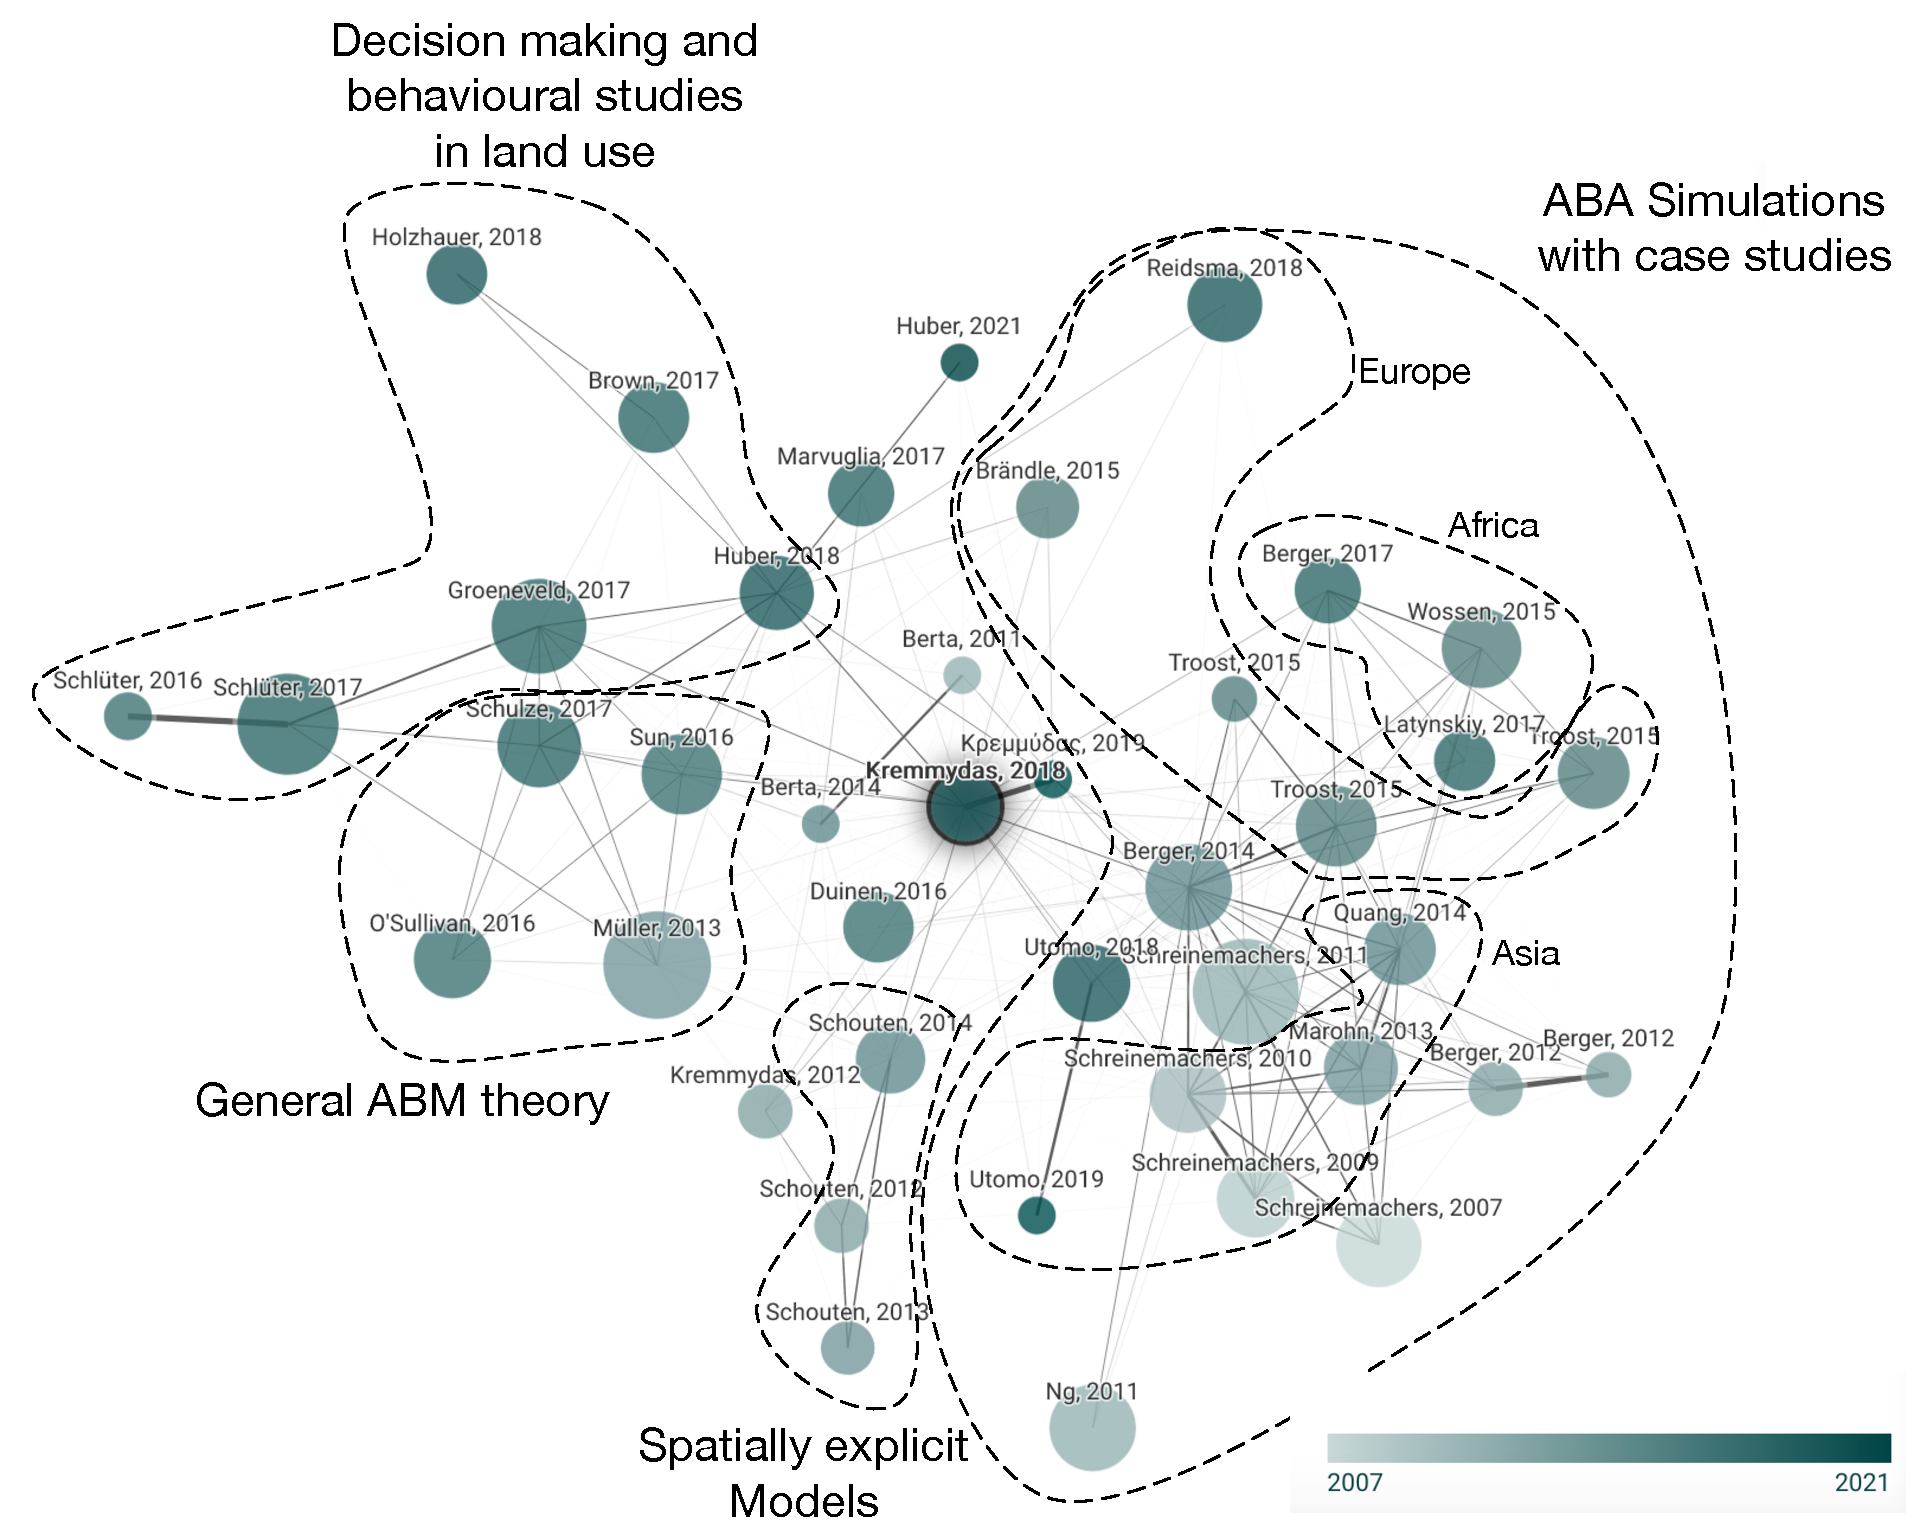
\includegraphics[width=.8\textwidth]{Figures/StateOfTheArt2.pdf}
	\centering
	\caption{\small Graph showing papers related to ref. \cite{kremmydasReviewAgentBased2018} generated on \href{https://www.connectedpapers.com/main/35fac7b643317e5f48f5280fadec94051bf2401f/A-review-of-Agent-Based-Modeling-for-agricultural-policy-evaluation/graph}{Connected Papers}. Circle radius is proportional to number of citation, color to publication date, dashed line refers to paper categories. ABM: agent-based modelling, ABA: agent-based agricultural simulations.}
	\label{fig:State_of_the_art}
\end{figure}

\section{The Crop War model}

\subsection{Software}
In order to build the model, we decided to use the python library \href{https://agentpy.readthedocs.io/en/stable/overview.html}{Agentpy} which conveniently introduces the \texttt{Agent}, \texttt{Grid}, \texttt{Model}, and \texttt{Experiment} classes, allowing to create our model with minimal pre-requisite work.\\
The present report was generated via LaTeX, and all relevant programs or documents were hosted on a git repo, with which our team interacted using Visual Studio Code.

\subsection{Overview}

The Crop War model aims to visualise how farmers can compete with respect to water ressources and crop profitability, given a geogaphical environment (the \texttt{Map} class) and a set of externalities including weather conditions, market dynamics (supply and demand impacting the price of crops), variable water ressources and government policies.

At each time step $dt$, all agents collect their crop yields and are faced with the choice of selling it at market price or stocking it for later use. Agents can also change the crops they are growing, or leave their land idle for replenishment of its nutritive properties, where the respective probabilities of these choices can be influenced by agent personalities.\\
The wealth $W_i$ of each agent is then plotted as a function of time $t$, and an analyis is carried out to explain the success rate of different strategies, given a set of externalities such as weather conditions or government policies.

\subsection{Model development}
In order to illustrate the development of our Crop Wars model, this section is organised in versions, starting from the simple, deterministic \tagg{v1.0} on top of which we progressively implement new features such as market dynamics, weather events and agent personalities.

\subsubsection{Version 1.0}
The first version of the model is not spatially resolved, in the sense that each agent can only grow one crop at a time and can not expand to other locations.\\
The price of each crop is fixed and does not vary as a function of time, and the agents only have the choice between selling or stocking their yields, their storage space being unlimited.\\
Fig. show the evolution of the budget (in \$) and stock as a function of time over 10 time steps for 5 agents choosing between 2 crops to grow:


\pgfplotstableread[col sep=comma]{Data/v10_budget.csv}{\budgeta}
\pgfplotstableread[col sep=comma, skip first n=3]{Data/v10_stock.csv}{\stocka}


%figure showing 4 subfigures: wealth, crop stocks (1 and 2) and the map
\begin{figure}[H]
	%wealth
\begin{subfigure}[hb]{0.45\textwidth}
	\resizebox{\linewidth}{!}{
		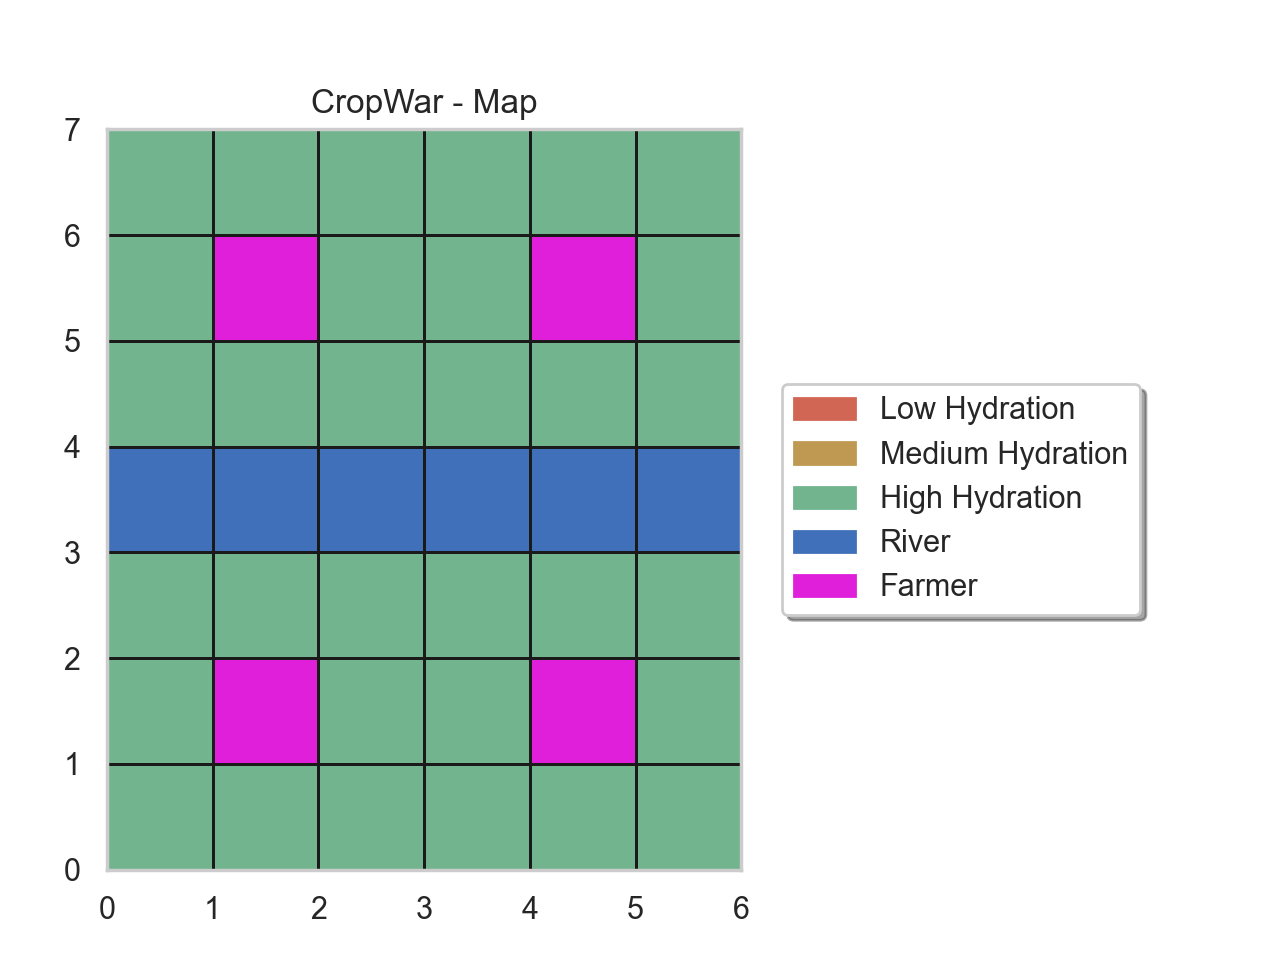
\includegraphics[width=\textwidth]{Figures/v01_Map.png}
	}
\end{subfigure}
\hfill
%crop 1
\begin{subfigure}[hb]{0.5\textwidth}
	\resizebox{\linewidth}{!}{\begin{tikzpicture}
		\pgfplotsset{
			scale only axis,
		}
		%axis options:
		\begin{axis}[
		  xlabel=Time step (years),
		  ylabel=Farmer wealth (\$),
		  xmin=0,
		  ymin=350,
		  legend pos=south east
		]
		  %plot 1: farmer ID 1
		  \addplot[
			  color={rgb:red,3;green,1;blue,2},
			  no marks,
			  thick
				  ] 
			  table[y index =1]{\budgeta};
		  \addlegendentry{$1$}
		  
		  %plot 2: farmer ID 2
		  \addplot[
			  color={rgb:red,1;green,1;blue,2},
			  dashed,
			  thick,
			  rounded corners
				  ]  table[y index =2]{\budgeta};
		  \addlegendentry{$2$}
  
		  %plot 3: farmer ID 3
		  \addplot[
			  color={rgb:red,0;green,3;blue,1},
			  loosely dotted,
			  mark = x
				  ] table[y index =3]{\budgeta};
		  \addlegendentry{$3$}
  
		  %plot 4: farmer ID 4
		  \addplot[
			  color={rgb:red,3;green,0;blue,2},
			  no marks,
			  rounded corners,
			  thick
				  ] table[y index =4]{\budgeta};
		  \addlegendentry{$4$}
  
		\end{axis}
	  \end{tikzpicture}
	  }
\end{subfigure}
\newline
%crop 1
\begin{subfigure}[hb]{0.5\textwidth}
	\resizebox{\linewidth}{!}{\begin{tikzpicture}
		\pgfplotsset{
			scale only axis,
		}
	  
		\begin{axis}[
		  xlabel=Time step (years),
		  ylabel=Farmer stock,
		  xmin=0,
		  ymin=0,
		  legend pos=north west
		]
		  %plot 1: farmer ID 1
	  \addplot[
		  color={rgb:red,3;green,1;blue,2},
		  no marks,
		  rounded corners
			  ] table[y index =1]{\stocka};
	  \addlegendentry{$1$}
	  
	  %plot 2: farmer ID 2
	  \addplot[
		  color={rgb:red,1;green,1;blue,2},
		  no marks
			  ]  table[y index =2]{\stocka};
	  \addlegendentry{$2$}

	  %plot 3: farmer ID 3
	  \addplot[
		  color={rgb:red,0;green,3;blue,1},
		  dashed,
		  mark = x
			  ] table[y index =3]{\stocka};
	  \addlegendentry{$3$}

	  %plot 4: farmer ID 4
	  \addplot[
		  color={rgb:red,3;green,0;blue,2},
		  no marks,
		  rounded corners
			  ] table[y index =4]{\stocka};
	  \addlegendentry{$4$}

	  \end{axis}
	  \end{tikzpicture}
  }
\end{subfigure}
\begin{subfigure}[hb]{0.5\textwidth}
	\resizebox{\linewidth}{!}{\begin{tikzpicture}
		\pgfplotsset{
			scale only axis,
		}
	  
		\begin{axis}[
		  xlabel=Time step (years),
		  ylabel=Farmer stock,
		  xmin=0,
		  ymin=0,
		  legend pos=north west
		]

		  \addplot table[y index =5]{\stocka};
		  \addlegendentry{$1$}
		  \addplot table[y index =6]{\stocka};
		  \addlegendentry{$2$}
		  \addplot table[y index =7]{\stocka};
		  \addlegendentry{$3$}
		  \addplot table[y index =8]{\stocka};
		  \addlegendentry{$4$}
		\end{axis}
	  \end{tikzpicture}
  }
\end{subfigure}
\caption{Graph showing the map with four farmers, the evolution of crop stocks the and farmer's budget as a function of time over 10 time steps}
\end{figure}


\subsubsection{Version 1.2}
In the second version of the model \tagg{v1.2}, the agents can expand to neighbouring cells in order to grow more crops.


\pgfplotstableread[col sep=comma]{Data/v12_budget.csv}{\budgetb}
\pgfplotstableread[col sep=comma, skip first n=3]{Data/v12_stock.csv}{\stockb}



\subsection{The market model}

\subsection{Agent strategies}



%command to display code:
%\begin{lstlisting}
%\end{lstlisting}


\newpage
\bibliographystyle{ieeetr} 
\bibliography{AgentBasedModelling.bib}

\end{document}
